\section{Correlation}

Correlation is the foundational premise of predictive modeling, in the sense that it provides a quantitative basis upon which we can forecast future outcomes.

A strong correlation between two variables suggests the existence of a mutual dependence between them: if one variable undergoes a change, the other variable will systematically change as well.

We can state that a strong correlation guarantees a mathematical relationship between two variables, and because of this structure, we will be able to predict their combined behavior.

This relationship can assume any functional form. If $X$ and $Y$ are two correlated variables, we can express their linkage mathematically as:
\begin{align}
	Y = f(X)
\end{align}

\subsection{Examples of Correlation}
\begin{itemize}
	\item Linear correlation:
	\begin{align}
		y = ax + b
	\end{align}
	\item Exponential correlation:
	\begin{align}
		y = be^{ax}
	\end{align}
\end{itemize}

\subsection{Definition of Correlation}
If $X$ and $Y$ are two discrete random variables that can take values $\set{x_0, x_1, \dots}$ and $\set{y_0, y_1, \dots}$ with arithmetic averages $\bar{x}$ and $\bar{y}$ respectively, their correlation coefficient is defined as:
\begin{align}
	\corr(X,Y) = \dfrac{\sum_{x_i, y_j} \left( (x_i - \bar{x})(y_j - \bar{y}) \right)}{\sqrt{\sum_{x_i, y_j} (x_i - \bar{x})^2 \sum_{x_i, y_j} (y_j - \bar{y})^2}}
\end{align}

\subsection{Properties of Correlation}
\begin{itemize}
	\item The value of the correlation coefficient is strictly bounded between $-1$ and $1$; that is, $-1 \leq \corr(X,Y) \leq 1$.
	\item A positive correlation indicates a direct relationship between the two variables (both increase or decrease together).
	\item A negative correlation indicates an inverse relationship between the two variables (as one increases, the other decreases).
	\item The closer the absolute magnitude of the coefficient is to $1$, the stronger and tighter the empirical relationship between the variables.
\end{itemize}

\subsection{Warning!}
Although a strong correlation suggests some form of structural relationship that can be leveraged to predict the behavior of one variable given another, \emph{this does not imply that such a relationship is the sole causal factor explaining that behavior.}

\begin{observacion}
	\emph{Correlation does not imply causation!}
\end{observacion}

For instance, there exists a very strong positive correlation between the number of vocabulary words known by a human being and their shoe size. However, this empirical linkage is easily explained by a confounding demographic factor: as children grow older, they naturally require larger shoes and simultaneously acquire new vocabulary.

\emph{This certainly does not mean that wearing larger shoes will make a person more cultured or intelligent!}

Let us endeavor to understand this concept more concretely by exploring a dataset and attempting to uncover correlations among its variables. The dataset we will examine is a well-known benchmark detailing miscellaneous financial expenditures incurred in \emph{advertising across various media platforms} and the resulting \emph{sales volume of a particular product.}

Subsequently, we will employ the quantitative framework known as \emph{linear regression} to rigorously model these exact same data.

For now, let us import this dataset and compute its pairwise correlation coefficients:

[,]{\texttt{advertising.py}}
\begin{lstlisting}[language=Python]
#!/usr/bin/env python3
# -*- coding: utf-8 -*-

import pandas as pd

advert = pd.read_csv("./dataBases/Advertising.csv")
print(advert.head())

import numpy as np

advert["dX*dY"] = (advert["TV"] - np.mean(advert["TV"])) * (advert["Sales"] - np.mean(advert["Sales"]))
advert["dX**2"] = (advert["TV"] - np.mean(advert["TV"])) ** 2
advert["dY**2"] = (advert["Sales"] - np.mean(advert["Sales"])) ** 2

sxy = advert.sum()["dX*dY"]
sxx = advert.sum()["dX**2"]
syy = advert.sum()["dY**2"]

r = sxy / np.sqrt(sxx * syy)
\end{lstlisting}

[,]{Screen Output}
\begin{lstlisting}[language=Python]
   TV  Radio  Newspaper  Sales
0  230.1   37.8       69.2   22.1
1   44.5   39.3       45.1   10.4
2   17.2   45.9       69.3    9.3
3  151.5   41.3       58.5   18.5
4  180.8   10.8       58.4   12.9
\end{lstlisting}

[,]{\texttt{advertising2.py}}
\begin{lstlisting}[language=Python]
#!/usr/bin/env python3
# -*- coding: utf-8 -*-

import pandas as pd
advert = pd.read_csv("./dataBases/Advertising.csv")
print(advert.head())

import numpy as np

def rCoef(df, var1, var2):
    df["dX*dY"] = (df[var1] - np.mean(df[var1])) * (df[var2] - np.mean(df[var2]))
    df["dX**2"] = (df[var1] - np.mean(df[var1])) ** 2
    df["dY**2"] = (df[var2] - np.mean(df[var2])) ** 2
    sxy = df.sum()["dX*dY"]
    sxx = df.sum()["dX**2"]
    syy = df.sum()["dY**2"]
    r = sxy / np.sqrt(sxx * syy)
    return r

tvVsSales = rCoef(advert, "TV", "Sales")
## 0.782224424862
radioVsSales = rCoef(advert, "Radio", "Sales")
## 0.576222574571
\end{lstlisting}

\begin{figure}
	\centering
	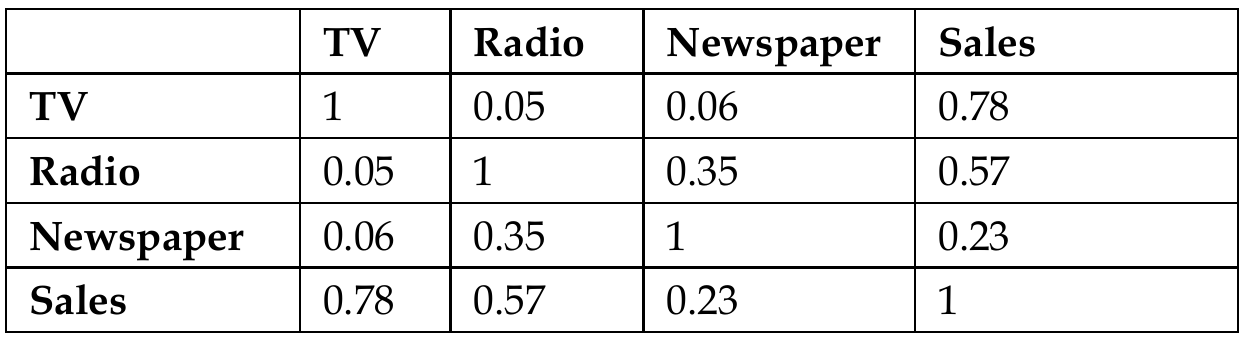
\includegraphics[width=10cm,keepaspectratio=true]{./images/correlationMatrix.png}
	\caption{Correlation matrix}
	\label{correlationMatrix}
\end{figure}

Let us visually examine the nature of these correlations by plotting the variables \texttt{TV}, \texttt{Radio}, and \texttt{Newspaper} versus \texttt{Sales} from the \texttt{advert} data frame.

[,]{tvVsSales.py}
\begin{lstlisting}[language=Python]
#!/usr/bin/env python3
# -*- coding: utf-8 -*-

import pandas as pd
advert = pd.read_csv("./dataBases/Advertising.csv")

import matplotlib.pyplot as plt

plt.plot(advert['TV'], advert['Sales'], 'ro')
plt.title('TV vs Sales')
plt.show()

plt.plot(advert['Radio'], advert['Sales'], 'ro')
plt.title('Radio vs Sales')
plt.show()

plt.plot(advert['Newspaper'], advert['Sales'], 'ro')
plt.title('Newspaper vs Sales')
plt.show()
\end{lstlisting}

\begin{center}
	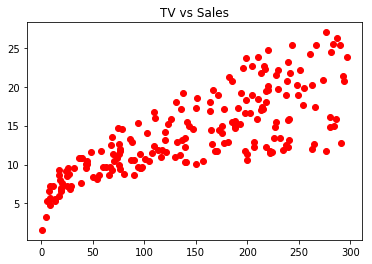
\includegraphics[width=10cm,keepaspectratio=true]{./images/tvVsSales.png}
\end{center}

\begin{center}
	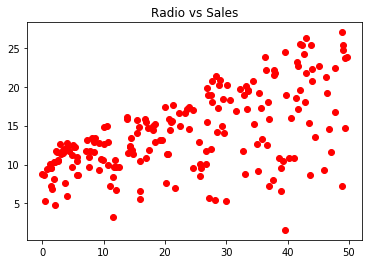
\includegraphics[width=10cm,keepaspectratio=true]{./images/radioVsSales.png}
\end{center}

\begin{center}
	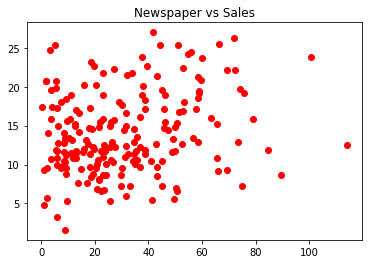
\includegraphics[width=10cm,keepaspectratio=true]{./images/newsVsSales.png}
\end{center}
